\documentclass[aspectratio=169]{beamer}
\usepackage{amsmath, amssymb, amsfonts, amsthm}
\usepackage{cancel}
\usepackage[output-complex-root=j]{siunitx}
\usepackage[american, nooldvoltagedirection]{circuitikz}
\usepackage{bm}
\usepackage{listings}
\usepackage{graphicx}
\usepackage{hyperref}

\usetheme{Berkeley}
\usefonttheme[onlymath]{serif}
\AtBeginSection[]{
    \begin{frame}
    \vfill
    \centering
    \begin{beamercolorbox}[sep=8pt,center,shadow=false,rounded=false]{title}
    \usebeamerfont{title}\insertsectionhead\par
    \end{beamercolorbox}
    \vfill
    \end{frame}
}

\newcommand{\N}{\mathbb{N}}
\newcommand{\Z}{\mathbb{Z}}
\newcommand{\Q}{\mathbb{Q}}
\newcommand{\R}{\mathbb{R}}
\renewcommand{\C}{\mathbb{C}}

\title{EECS 16B CSM}
\author{Bryan Ngo}
\date{2020-11-30}
\institute{UC Berkeley}

\begin{document}

\begin{frame}
    \maketitle
\end{frame}

\begin{frame}
    \frametitle{Convolutions}
    \framesubtitle{Definition}

    \begin{equation}
        (f \ast g)[n] = \sum_{m \in \Z} f[m] g[n - m]
    \end{equation}
    \begin{itemize}
        \item only works with LTI systems
        \item "flip and drag" technique
        \item commutative, associative, distributive over addition
    \end{itemize}
\end{frame}

\begin{frame}
    \frametitle{Convolutions}
    \framesubtitle{Visual}

    \begin{center}
        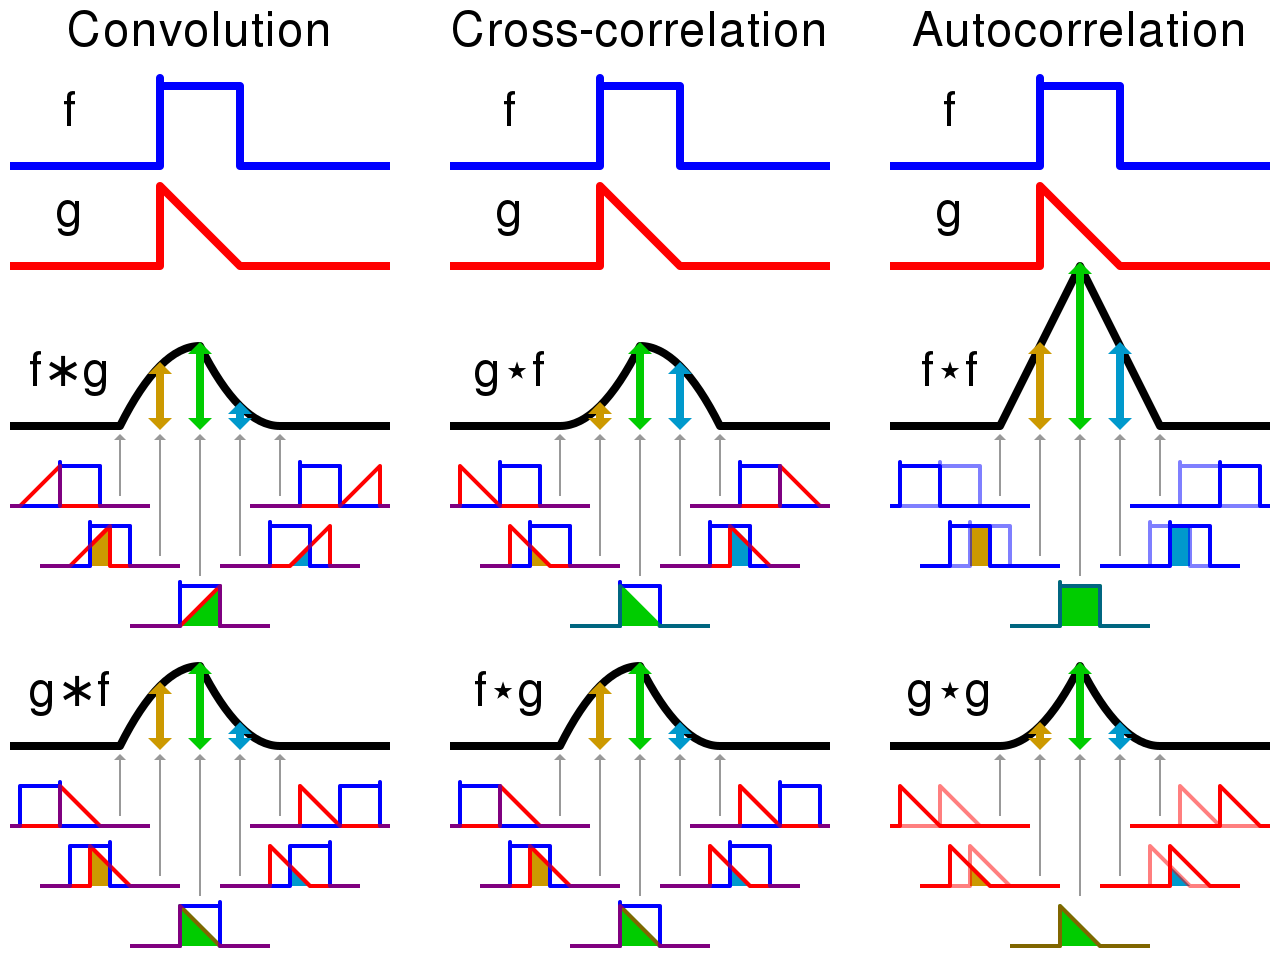
\includegraphics[height=0.8\textheight]{Comparison_convolution_correlation.svg.png}
    \end{center}
\end{frame}

\begin{frame}
    \frametitle{Convolutions}
    \framesubtitle{Applications}

    \begin{center}
        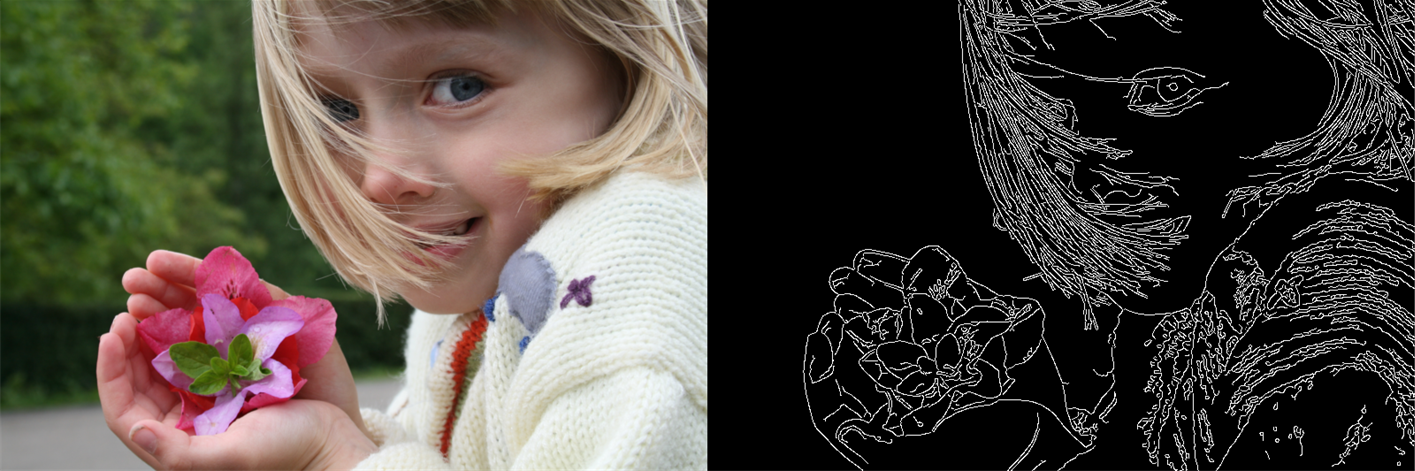
\includegraphics[height=0.5\textheight]{edge-detection.png}
    \end{center}
    \begin{itemize}
        \item \href{https://towardsdatascience.com/intuitively-understanding-convolutions-for-deep-learning-1f6f42faee1}{2D convolution}
        \item image processing (edge detection)
        \item signal processing
        \item \href{https://youtu.be/8rrHTtUzyZA?list=PLP8iPy9hna6Q2Kr16aWPOKE0dz9OnsnIJ}{3b1b guy on convolutions}
    \end{itemize}
\end{frame}

\begin{frame}
    \frametitle{Discrete Fourier Transform}

    \begin{center}
        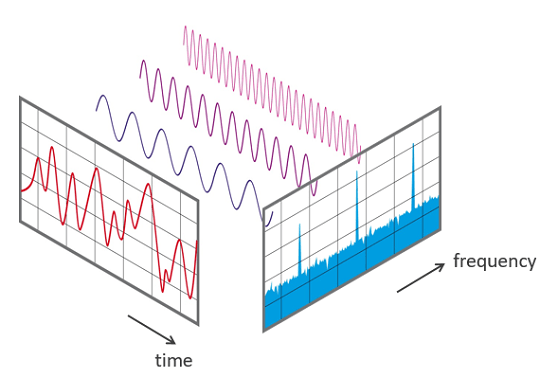
\includegraphics[height=0.5\textheight]{fourier.png}
    \end{center}
    \begin{equation}
        X(\omega) = \frac{1}{\sqrt{N}} \sum_{n \in [0, N - 1]} x[n] e^{-j \omega n}
    \end{equation}
    \begin{itemize}
        \item splits up a signal into its constituent frequencies
        \item \href{https://youtu.be/spUNpyF58BY}{3b1b video on CFT}
    \end{itemize}
\end{frame}

\end{document}
